%=========================================================
\chapter{Modelo del Negocio}	
\label{cap:reqSist}

	En este capítulo se modela la {\em Arquitectura del negocio} la cual está conformada por la Ontología del negocio ({\em Términos} y {\em Hechos del negocio}), Arquitectura de procesos y las {\em Reglas del negocio}. Primero se especifica brevemente el {\em Contexto} en el que los términos tienen significado.
	
	En las secciones \ref{sec:terminosDeNegocio} y \ref{sec:hechosDeNegocio} se presentan los Términos del negocio a manera de Glosario y por último se presentan los Hechos del negocio a manera de relaciones entre términos del negocio.

%----------------------------------------------------------
\section{Contexto}

	La empresa ``Guarderia Burbujas'' se dedica a el cuidado y atencion de infantes. Su principal objetivo es brindar un entorno seguro, educativo y estimulante para el desarrollo integral de los niños mientras sus padres trabajan o realizan otras actividades.
    La guarderia cuenta con salas en donde se quedan los infantes, mientras tres docentes los estan cuidando y realizando actividades con ellos, si alguninfante tiene que ir a hacer una evacuacion un profesor lo acompaña y los otros dos se quedan vigilando a los demas infantes.
    Tambien se cuenta con un nutriologo en cargado de mantener a los infantes con una dieta balanceada y con un medico engargado de atender cualquier incidente medico que ocurra dentro de la guarderia.
	
%---------------------------------------------------------
\section{Términos del Negocio}
\label{sec:terminosDeNegocio}

\begin{description}
	\item[\hypertarget{tusuario}{Usuario:}] Persona fisica que tienen acceso al sistema. 
 
	\item[\hypertarget{tinfante}{Infante:}] Se refiere a las personad de entre 3 meses y 6 años que asisten a la guarderia.
	
	\item[\hypertarget{tDocente}{Profesor:}] Tipo de Usuario que esta al frente de una sala para cuidar a los infantes y dejarles actividades ludicas, asi como para estar al pendiente de sus ingestas y evacuaciones.
 
	\item[\hypertarget{treporte}{Reporte:}] Documento con el cual se le informa a los padres de familia las actividades que ha realizado su hijo durante el dia, como sus ingestas, evacuaciones y si hubo alcun incidente con su hijo.
	
	\item[\hypertarget{tEvento}{Evento:}] Acontecimientos relevantes en la guarderia como festivales, convivios o dias inhabiles.
	
	\item[\hypertarget{ttarea}{Tarea:}] Actividad que los profesores dejan a los infantes para que las realicen en casa con el proposito de reforzar lo visto en la guarderia. 

	\item[\hypertarget{tactividad}{Actividad:}] Se refiere a toda accion que el profesor solicita a los infantes que realicen durante su estandia en la guarderia con proposito educativo y que favorece el desarrollo del infante.
	
	\item[\hypertarget{tMenu}{Menu:}] Documento en el cual se puede visualizar las comidas de todo un mes de los infantes.

        \item[\hypertarget{tIngesta}{Ingesta:}] Material alimenticio o líquidos que se incorporan al organismo por la boca en un periodo determinado.

        \item[\hypertarget{tEvacuacion}{Evacuacion:}] Materia compuesta de residuos de alimento que el organismo elimina tras haber hecho la digestión.
        
        \item[\hypertarget{tNutriologo}{Nutriologo:}] Usuario encargado de hacer la planificacion del menu de los infantes, cuidando que tengan una dieta balanceada.
        
	
        \item[\hypertarget{tSala}{Sala:}] Lugar en la guarderia destinado a los infantes.

        
        \item[\hypertarget{tpadre}{Padre de familia:}] Engargado legal de un infante.

        
        \item[\hypertarget{tMedico}{medico:}] Usuario con licencia medica que Se encarga de atender temas de salud de los infantes.

        
        \item[\hypertarget{tdirector}{Director:}] Autoridad de la guarderia, se encarga de organizar los eventos escolares y los dias inhabiles.
        
%	\brTermSensor{tVelocimetro}{Velocímetro:}{Velocidad de un Vehículo.}{Kilometros/hora.}{Constantemente siempre que el \cdtRef{tVehiculo}{vehículo} esté encendido.}
\end{description}


\newpage
%----------------------------------------------------------
\section{Modelo del dominio del problema}
\label{sec:hechosDeNegocio}


%- - - - - - - - - - - - - - - - - - - - - - - - - - - - - 
\subsection{Modelo del dominio del problema}

	El modelo del dominio del problema se muestra en la figura~\ref{fig:modeloDeDominio}, a continuación se describen cada una de las entidades y sus relaciones.
	
\begin{figure}[htbp!]
	\begin{center}
		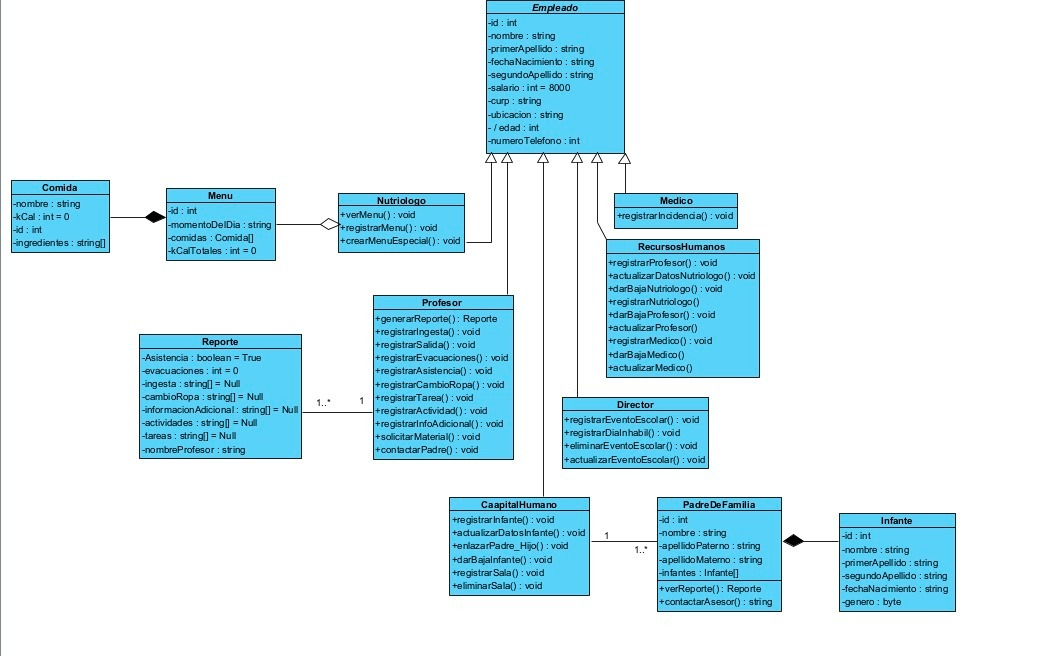
\includegraphics[angle=90,width=.58\textwidth]{images/diagramaClases.jpeg}
		\caption{Modelo del dominio del problema}
		\label{fig:modeloDeDominio}
	\end{center}
\end{figure}


\newpage
\begin{cdtEntidad}{infante}{Infante}
	\brAttr{id}{Id}{Id}{Número de registro utilizado para identificar un alumno}{Sí}
	\brAttr{nombre}{Nombre}{Palabra Corta}
		{Nombre o nombres del alumno.}{Sí}
	\brAttr{primerApellido}{Primer apellido}{Palabra Corta}
		{Primer apellido del alumno.}{Sí}
	\brAttr{segundoApellido}{Segundo apellido}{Palabra Corta}
		{Segundo apellido del alumno.}{No}
	\brAttr{nacimiento}{FechaNacimiento}{Fecha}
		{Fecha de nacimiento del alumno.}{Sí}
	\brAttr{genero}{Género}{byte}
		{Género del alumno.}{No}
\end{cdtEntidad}

%- - - - - - - - - - - - - - - - - - - - - - - - - - - - - 
\begin{cdtEntidad}{padredefamilia}{Padre de Familia}%{}
	\brAttr{id}{Id}{Id}{Número de registro utilizado para identificar un alumno}{Sí}
	\brAttr{nombre}{Nombre}{Palabra Corta}
		{Nombre o nombres del alumno.}{Sí}
	\brAttr{primerApellido}{Primer apellido}{Palabra Corta}
		{Primer apellido del alumno.}{Sí}
	\brAttr{segundoApellido}{Segundo apellido}{Palabra Corta}
		{Segundo apellido del alumno.}{No}
	\brAttr{infantes}{Infantes}{Lista}
		{Lista de todos los infantes a su cargo.}{Sí}
	\brAttr{reportes}{Reportes}{Lista}
		{Lista de todos los reportes de los infantes que tiene a cargo el padre de familia.}{No}
        \brAttr{citas}{Citas}{Lista}{Lista de todas las citas que tiene el padre de familia}{No}
	\cdtEntityRelSection
	\brRel{\brRelComposition}{Infante}{Un \hyperlink{padredefamilia}{Padre de familia} tiene \hyperlink{infante}{Infantes} a su cargo}	
	\brRel{\brRelComposition}{Citas}{Un \hyperlink{padredefamilia}{Padre de familia} tiene  \hyperlink{citas}{citas} a las que asistir}
        \brRel{\brRelComposition}{Reporte}{un \hyperlink{padredefamilia}{Padre de familia} tiene los \hyperlink{reporte}{reportes} de sus infantes}
\end{cdtEntidad}

%---------------------------------------------------------
\newpage
\begin{cdtEntidad}{citas}{Citas}
	\brAttr{fecha}{Fecha}{Fecha}{Fecha en la que la cita esta programada}{Sí}
	\brAttr{nombreinfante}{NombreInfante}{Palabra Corta}
		{Nombre del alumno.}{Sí}
	\brAttr{nombrepadre}{NombrePadre}{Palabra Corta}
		{nombre del padre del infante.}{Sí}
	\brAttr{hora}{Hora}{time}
		{Hora en la que la cita esta programada.}{Si}
	\brAttr{id}{ID}{byte}
		{Numero de registro utilizado para identificar la cita.}{Sí}
\end{cdtEntidad}

%- - - - - - - - - - - - - - - - - - - - - - - - - - - - - 
\begin{cdtEntidad}{Reportes}{Reportes}
	\brAttr{asistencia}{Asistencia}{Boolean}{muestra si el infante asistio un dia}{Sí}
	\brAttr{evacuaciones}{Evacuaciones}{Int}
		{muestra la cantidad de veces que el infante evacuó.}{Sí}
	\brAttr{ingesta}{Ingesta}{Palabra Corta}
		{Muestra la cantidad de comida que ingirio el infante.}{Sí}
	\brAttr{cambioropa}{CambioRopa}{Palabra Corta}
		{Muestra cuantos cambios de ropa uso el infante y cuantos tiene aun disponibles.}{No}
	\brAttr{informacionadicional}{Informacion Adicional}{String}
		{Muestra otra informacion que se considere relevante sobre el infante.}{Sí}
	\brAttr{actividades}{Actividades}{String}
		{Muestra las actividades realizadas por el alumno.}{No}
        \brAttr{tareas}{Tareas}{String}{Muestra las tareas que debe realizar el padre de familia con el infante}{No}
        \brAttr{nombreprofesor}{Nombre Profesor}{palara corta}{Muestra el nombre del profesor que realizo el reporte}{Si}
\end{cdtEntidad}

%- - - - - - - - - - - - - - - - - - - - - - - - - - - - - 
\begin{cdtEntidad}{comida}{Comida}
	\brAttr{nombre}{Nombre}{Palabra corta}{nombre del platillo}{Sí}
	\brAttr{kcal}{Kcal}{Int}
		{muestra la cantidad de kilo calorias que el platillo aporta.}{Sí}
	\brAttr{ingredientes}{Ingredientes}{String}
		{Muestra los ingredientes con los que se prepara una comida.}{No}
	\brAttr{id}{Id}{int}
		{Numero de registro con el que se identifica al platillo.}{Sí}
\end{cdtEntidad}
%- - - - - - - - - - - - - - - - - - - - - - - - - - - - - 
\newpage
\section{Modelado de Reglas de negocio}

\begin{BussinesRule}{RN1}{Fecha de Nacimiento correcta.}
	\BRitem[Tipo:] Regla de integridad referencial o estructural. 
				% Otras opciones para tipo: 
				% - Regla de integridad referencial o estructural. 
				% - Regla de operación, (calcular o determinar un valor.).
				% - Regla de inferencia de un hecho.
	\BRitem[Clase:] Habilitadora. 
				% Otras opciones para clase: Habilitadora, Cronometrada, Ejecutive.
	\BRitem[Nivel:] Control. % Otras opciones para nivel: Control, Influencia.
	\BRitem[Descripción:]	Las Fechas de Nacimiento de los infantes debe ser mayores al día Primero de Enero del año 2018 y menor a tres meses antes de la fecha actual.
	\BRitem[Motivación:] Evitar fraudes al PRONIM por el registro de personas que no han nacido al momento de su registro.
	\BRitem[Sentencia:] $\forall p \in Persona \Rightarrow 01-Enero-2018~<~p.fechaDeNacimiento~<~fechaActual menos 3 meses$.
	\BRitem[Ejemplo positivo:] Para el día 23 de Junio del 2023, cumplen la regla: 		
        \begin{itemize}
        	\item 11 de Octubre del 2020
			\item 20 de Diciembre del 2021
			\item 2 de Enero del 2023
        \end{itemize}
	
	\BRitem[Ejemplo negativo:] Para el día 23 de Junio del 2013, no cumplen la 
		\begin{itemize}
        	\item 12 de junio del 2013
			\item 20 de Diciembre del 2014
			\item 1 de Enero del 1900
			\item 31 de Diciembre del 2024
        \end{itemize}
	
	\BRitem[Referenciado por:] \hyperlink{CU3}{CU3}.
\end{BussinesRule}

\begin{BussinesRule}{RN2}{Atencion medica.} 
	\BRitem[Tipo:] Regla de Condicion. 
				% Otras opciones para tipo: 
				% - Regla de integridad referencial o estructural. 
				% - Regla de operación, (calcular o determinar un valor.).
				% - Regla de inferencia de un hecho.
	\BRitem[Clase:] Habilitadora. 
				% Otras opciones para clase: Habilitadora, Cronometrada, Ejecutive.
	\BRitem[Nivel:] Control. % Otras opciones para nivel: Control, Influencia.
	\BRitem[Descripción:] Cuando un infante requiera atencion medica de bajo nivel , el medico debe atenderlo de manera oportina, ademas de registrar el reporte de la incidencia medica.
        \BRitem[Motivación:] Garantiza el cuidado oportuno de los infantes, ademas de que notifica a los padres de familia cuando ocurre algo con sus hijos.
	\BRitem[Ejemplo positivo:] 
                \begin{itemize}
                    \item Juan se resbaló en el ultimo escalon, por lo que golpeo su cabeza, por lo que fue revisado por el medico para descartar una contucion y registra el reporte del incidente.
                \end{itemize}
	\BRitem[Ejemplo negativo:] 
                \begin{itemize}
                    \item Pedro se cayo y se raspo la rodilla, por lo que el medico le lavo la herida pero no realizo el reporte
	        \end{itemize}
         
	\BRitem[Referenciado por:] \hyperlink{CU15}{CU15}.
\end{BussinesRule}

\begin{BussinesRule}{RN3}{Notificacion de tareas}
	\BRitem[Tipo:] Regla de condicion.
				% Otras opciones para tipo: 
				% - Regla de integridad referencial o estructural. 
				% - Regla de operación, (calcular o determinar un valor.).
				% - Regla de inferencia de un hecho.
	\BRitem[Clase:] Habilitadora. 
				% Otras opciones para clase: Habilitadora, Cronometrada, Ejecutive.
	\BRitem[Nivel:] Influencia. % Otras opciones para nivel: Control, Influencia.
	\BRitem[Descripción:] Es responsabilidad del profesor dar a conocer las tareas que deberan hacer los infantes en sus casas para reforzar lo visto en el dia.
 
        \BRitem[Motivacion] Aumentar el desarrollo de los infantes, ademas de tener una buena comunicacion entre profesores y padres de familia
        
	\BRitem[Ejemplo positivo:] 
                \begin{itemize}
                    \item el profesor moises notifica a los padres de familia sobre todas las actividades que requiere que los infantes realicen en sus casa
                \end{itemize}
	
	\BRitem[Ejemplo negativo:] 
                \begin{itemize}
                    \item El profesor humberto no realiza la notificacion de tareas de los infantes, lo cual podria dificultar el progreso de los infantes
                \end{itemize}
 
	\BRitem[Referenciado por:] \hyperlink{CU12}{CU12}.
\end{BussinesRule}

\begin{BussinesRule}{BR4}{Toma de asistencia}
	\BRitem[Tipo:] Regla de integridad referencial o estructural.
				% Otras opciones para tipo: 
				% - Regla de integridad referencial o estructural. 
				% - Regla de operación, (calcular o determinar un valor.).
				% - Regla de inferencia de un hecho.
	\BRitem[Clase:] Habilitadora. 
				% Otras opciones para clase: Habilitadora, Cronometrada, Ejecutive.
	\BRitem[Nivel:] Control. % Otras opciones para nivel: Control, Influencia.
	\BRitem[Descripción:] Todos los profesores deberan tomar asistencia de los infantes todos los dias.
        \BRitem[Motivacion] Tener un control de cuando asistieron los infantes para poder mostrarlo a los padres de familia en caso de que se requiera
        
	\BRitem[Ejemplo positivo:] 
            \begin{itemize}
                \item El profesor ricardo pasa asistencia todos los dias a las 9:15
            \end{itemize}
	
	\BRitem[Ejemplo negativo:] 
	       \begin{itemize}
	           \item  El profesor humberto no pasa lista en la guarderia, pero cuando llega a su casa anota a los alumnos que recuerda que estuvieron.
	       \end{itemize}
	\BRitem[Referenciado por:] \hyperlink{CU19}{CU19} 
\end{BussinesRule}

\begin{BussinesRule}{RN5}{Asignacion de salas por edad}
	\BRitem[Tipo:] Regla de inferencia.
				% Otras opciones para tipo: 
				% - Regla de integridad referencial o estructural. 
				% - Regla de operación, (calcular o determinar un valor.).
				% - Regla de inferencia de un hecho.
	\BRitem[Clase:] Habilitadora. 
				% Otras opciones para clase: Habilitadora, Cronometrada, Ejecutive.
	\BRitem[Nivel:] Control. % Otras opciones para nivel: Control, Influencia.
	\BRitem[Descripción:] Los infantes seran asignados a salas basados en rangos de edades.
        \BRitem[Motivacion] Que los infantes tengan una buena interaccion social.
		
	\BRitem[Ejemplo positivo:] 
	        \begin{itemize}
	            \item Juanito de 7 meses fue asignado a una sala con infantes de 3 meses a 1 año 
	        \end{itemize}
	\BRitem[Ejemplo negativo:] 
	        \begin{itemize}
	            \item Juanito de 2 años fue asignado a una sala con infantes de 6 años
	        \end{itemize}
	\BRitem[Referenciado por: ]CU3 
\end{BussinesRule}

\begin{BussinesRule}{RN6}{Informar cantidad de ingesta}
	\BRitem[Tipo:] Inferencia de un hecho.
				% Otras opciones para tipo: 
				% - Regla de integridad referencial o estructural. 
				% - Regla de operación, (calcular o determinar un valor.).
				% - Regla de inferencia de un hecho.
	\BRitem[Clase:] Habilitadora. 
				% Otras opciones para clase: Habilitadora, Cronometrada, Ejecutive.
	\BRitem[Nivel:] Control. % Otras opciones para nivel: Control, Influencia.
	\BRitem[Descripción:] Los profesores deben de realizar el reporte de las cantidades de comida ingeridas por los infantes.
        \BRitem[Motivacion] Que los padres de familia esten informados acerca de la alimentacion de sus hijos
	\BRitem[Ejemplo positivo:] 
	        \begin{itemize}
	            \item El profesor alexis revisa cuanta comida queda en los platos de los infantes y anota cuanto comio cada quien, posteriormente registra las cantidades de comida ingeridas por los niños
	        \end{itemize}
	\BRitem[Ejemplo negativo:] 
	        \begin{itemize}
	            \item El profesor horacio no revisa cuanto come cada niño, y cuando le solicitan el reporte de ingestas registra que todos los niños acabaron toda su comida.
	        \end{itemize}
	\BRitem[Referenciado por:]CU9 
\end{BussinesRule}

\begin{BussinesRule}{RN7}{Informacion sobre eventos en la guarderia.}
	\BRitem[Tipo:] Regla de integridad.
				% Otras opciones para tipo: 
				% - Regla de integridad referencial o estructural. 
				% - Regla de operación, (calcular o determinar un valor.).
				% - Regla de inferencia de un hecho.
	\BRitem[Clase:] Habilitadora. 
				% Otras opciones para clase: Habilitadora, Cronometrada, Ejecutive.
	\BRitem[Nivel:] Control. % Otras opciones para nivel: Control, Influencia.
	\BRitem[Descripción:] El director debe notificar de todos los eventos academicos planeados a los padres de familia con al menos dos semanas de antelacion:
		
	\BRitem[Motivacion:] Que los padres de familia esten notificados de los eventos, teniendo sufuciente tiempo para saber si van a poder asistir, asi como de conseguir los materiales que se requieran.
	\BRitem[Ejemplo positivo:] 
	        \begin{itemize}
	            \item El director de la guarderia notifico el dia 21 de marzo que para el dia 10 de mayo se planea hacer un festival por el dia de las madres.
	        \end{itemize}
	\BRitem[Ejemplo negativo:] 
	        \begin{itemize}
	            \item El director de la guarderia notifica el 10 de septiembre que el dia 16 de septiembre tienen planeado realizar una kermes por el dia de la independencia
	        \end{itemize}
	\BRitem[Referenciado por:] CU17 
\end{BussinesRule}



%---------------------------------------------------------
